%%% Question %%%
% \begin{blocksection}
\begin{nonsol}
You can make the following analogy:
\begin{center}
\begin{tabular}{ |l|l| }
\hline
 \texttt{Link(1, Link.empty)} & \texttt{(cons 1 nil)} \\
 \texttt{a = Link(1, Link(2, Link.empty))} & \texttt{(define a (cons 1 (cons 2 nil)))}  \\
 \texttt{a.first} & \texttt{(car a)} \\
 \texttt{a.rest} & \texttt{(cdr a)} \\
 \hline
\end{tabular}

\end{center}
%Draw box and pointers when appropriate. Ask your mentor if you're unsure what's going on. You aren't expected to understand this completely on your own.
%\question What will Scheme output? Draw box-and-pointer diagrams to help determine this.
\end{nonsol}
\question What will Scheme output? Draw box and pointer diagrams where applicable.
\begin{lstlisting}
scm> (cons 1 (cons 2 nil))
\end{lstlisting}
\begin{solution}[0.25in]
\texttt{(1 2)}
\begin{center}
\includegraphics[scale=0.7]{scheme_lists_2}
\end{center}
\end{solution}

\begin{lstlisting}
scm> (cons 1 '(2 3 4 5))
\end{lstlisting}
\begin{solution}[0.25in]
\texttt{(1 2 3 4 5)}
\begin{center}
\includegraphics[scale=0.7]{scheme_lists_3}
When we use the quote before the list, we are saying that we should put the literal list (2 3 4 5) in the cdr of this list. So in this case we create a list where the first element (car) is 1, and the cdr is the list (2 3 4 5).
\end{center}
\end{solution}

\begin{lstlisting}
scm> (cons 1 '(2 (cons 3 nil)))
\end{lstlisting}
\begin{solution}[0.25in]
\texttt{(1 2 (cons 3 ()))}
\begin{center}
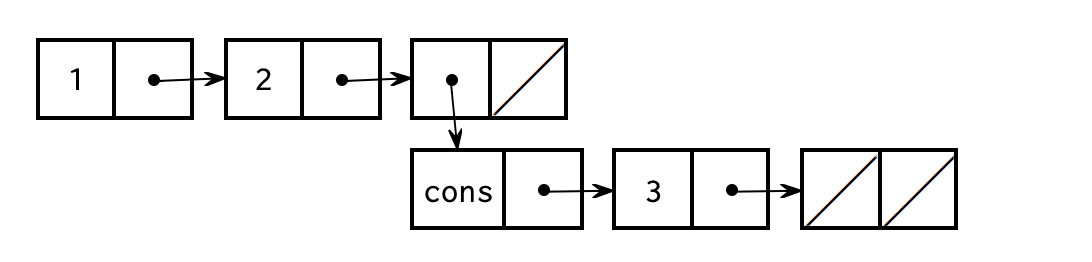
\includegraphics[scale=0.7]{scheme_lists_5}
Since we also used a quote here, we do not evaluate the \texttt{(cons 3 nil)}. We keep everything inside the quotes the same so the \texttt{cdr} of this list is the list \texttt{(2 (cons 3 nil))}. That means that we add the element 2, and then the nested list \texttt{(cons 3 nil)}.
\end{center}
\end{solution}

\begin{lstlisting}
scm> (cons 1 (2 (cons 3 nil)))
\end{lstlisting}
\begin{solution}[.25in]
\begin{lstlisting}
eval: bad function in : (2 (cons 3 nil))
\end{lstlisting}
While evaluating the operands, Scheme will try to evaluate the expression \texttt{(2 (cons 3 nil))}. Since 2 is not a valid operator, this expression Errors.
\end{solution}

\begin{lstlisting}
scm> (cons 3 (cons (cons 4 nil) nil))
\end{lstlisting}
\begin{solution}[.5in]
\lstinline$(3 (4))$
\end{solution}
% \end{blocksection}
% \begin{blocksection}
\begin{lstlisting}
scm> (define a '(1 2 3))
\end{lstlisting}
\begin{solution}[.25in]
\begin{lstlisting}
a
\end{lstlisting}
Defines a list of elements of \texttt{(1 2 3)} and binds the list to the variable \texttt{a}. Recall that define returns the name of the symbol.
\end{solution}

\begin{lstlisting}
scm> a
\end{lstlisting}
\begin{solution}[.25in]
\begin{lstlisting}
(1 2 3)
\end{lstlisting}
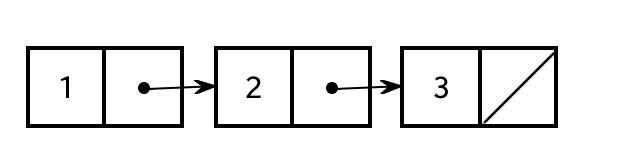
\includegraphics[scale=0.7]{scheme_lists_6}
\end{solution}

\begin{lstlisting}
scm> (car a)
\end{lstlisting}
\begin{solution}[.25in]
\begin{lstlisting}
1
\end{lstlisting}
\end{solution}

\begin{lstlisting}
scm> (cdr a)
\end{lstlisting}
\begin{solution}[.25in]
\begin{lstlisting}
(2 3)
\end{lstlisting}
\end{solution}

\begin{lstlisting}
scm> (cadr a)
\end{lstlisting}
\begin{solution}[.25in]
\begin{lstlisting}
2
\end{lstlisting}
Recall that cadr is short for \texttt{(car (cdr a))}. From above, we know that \texttt{(cdr a)} is \texttt{(2 3)}. From that, we can evaluate \texttt{(car (cdr a))} to 2.
\end{solution}

How can we get the 3 out of a?
\begin{solution}[.25in]
\begin{lstlisting}
(car (cdr (cdr a)))
\end{lstlisting}
To get to the pair that contains 3, we need to call \texttt{(cdr (cdr a))}. To get the element 3, we need the \texttt{car} of \texttt{(cdr (cdr a))}.
\end{solution}
% \end{blocksection}

\begin{blocksection}
\begin{guide}
\textbf{Teaching Tips}
\begin{itemize}
  \item Make sure students know \lstinline{(cadr a)} is short for \lstinline{(car (cdr a))} and \lstinline{(cddr a)} is short for \lstinline{(cdr (cdr a))}
  \item Draw diagrams or use the \href{https://code.cs61a.org/}{61A Scheme Web interpreter} for visualizing lists
  \item Encourage students to ask questions and experiment with extra \lstinline{cons}, \lstinline{car}, and \lstinline{cdr} statements to see how they change the outputs of statments!
  \item While unrelated to the problem, it may be helpful to teach students these keywords:
  \begin{itemize}
    \item\lstinline{(pair? arg)}, which checks if arg has a first and rest
    \item\lstinline{(list? arg)}, which returns true if arg is a well-formed list
  \end{itemize}
\end{itemize}
\end{guide}
\end{blocksection}
